% Created 2015-12-09 Wed 13:30
\documentclass[presentation, smaller]{beamer}
\usepackage[latin1]{inputenc}
\usepackage[T1]{fontenc}
\usepackage{fixltx2e}
\usepackage{graphicx}
\usepackage{longtable}
\usepackage{float}
\usepackage{wrapfig}
\usepackage{rotating}
\usepackage[normalem]{ulem}
\usepackage{amsmath}
\usepackage{textcomp}
\usepackage{marvosym}
\usepackage{wasysym}
\usepackage{amssymb}
\usepackage{hyperref}
\tolerance=1000
\mode<beamer>{\usetheme{Boadilla}\usecolortheme[RGB={40,100,30}]{structure}}
\usebackgroundtemplate{\includegraphics[width=\paperwidth]{MNRwhite}}
\setbeamersize{text margin left=10mm}
\usetheme{default}
\author{An Update}
\date{December 10, 2015.}
\title{FSIS-II}
\hypersetup{
  pdfkeywords={},
  pdfsubject={},
  pdfcreator={Emacs 24.3.1 (Org mode 8.2.10)}}
\begin{document}

\maketitle


\begin{frame}[label=sec-1]{Refresh of FSIS-II}
\begin{itemize}
\item available at: \url{http:\\142.143.160.56:8090}
\item Django 1.8.7
\item >90\% test coverage
\end{itemize}
\end{frame}

\begin{frame}[label=sec-2]{Updates include:}
\begin{itemize}
\item default view stocking in most recent year
\item better, more interactive maps
\item pages are 'save and send'
\item hatchery list has year range and quick-search
\item all cwts :
\begin{itemize}
\item all species in CWT\_Master.xls
\item including those from other jurisdictions
\end{itemize}
\end{itemize}
\end{frame}
\begin{frame}[label=sec-3]{Maps}
\begin{columns}
\begin{column}{0.4\textwidth}
\begin{itemize}
\item informative, context specific pop-up
\item some maps have tabs control what is displayed
\item 'Find Sites' and 'Find Events' save 'Region of Interest'
\begin{itemize}
\item editable with back-button
\end{itemize}
\end{itemize}
\end{column}
\begin{column}{0.6\textwidth}
\fbox{\includegraphics[width=0.9\textwidth]{example_map}}
\end{column}
\end{columns}
\end{frame}


\begin{frame}[label=sec-4]{Comments and Caveats}
\begin{columns}
\begin{column}{0.4\textwidth}

\begin{itemize}
\item still under development
\item interpret CWT recovery by Management Unit with caution - re-used
tags currently cause problems
\item Stocking events by strain by year not currently available
\end{itemize}
\end{column}

\begin{column}{0.6\textwidth}
\fbox{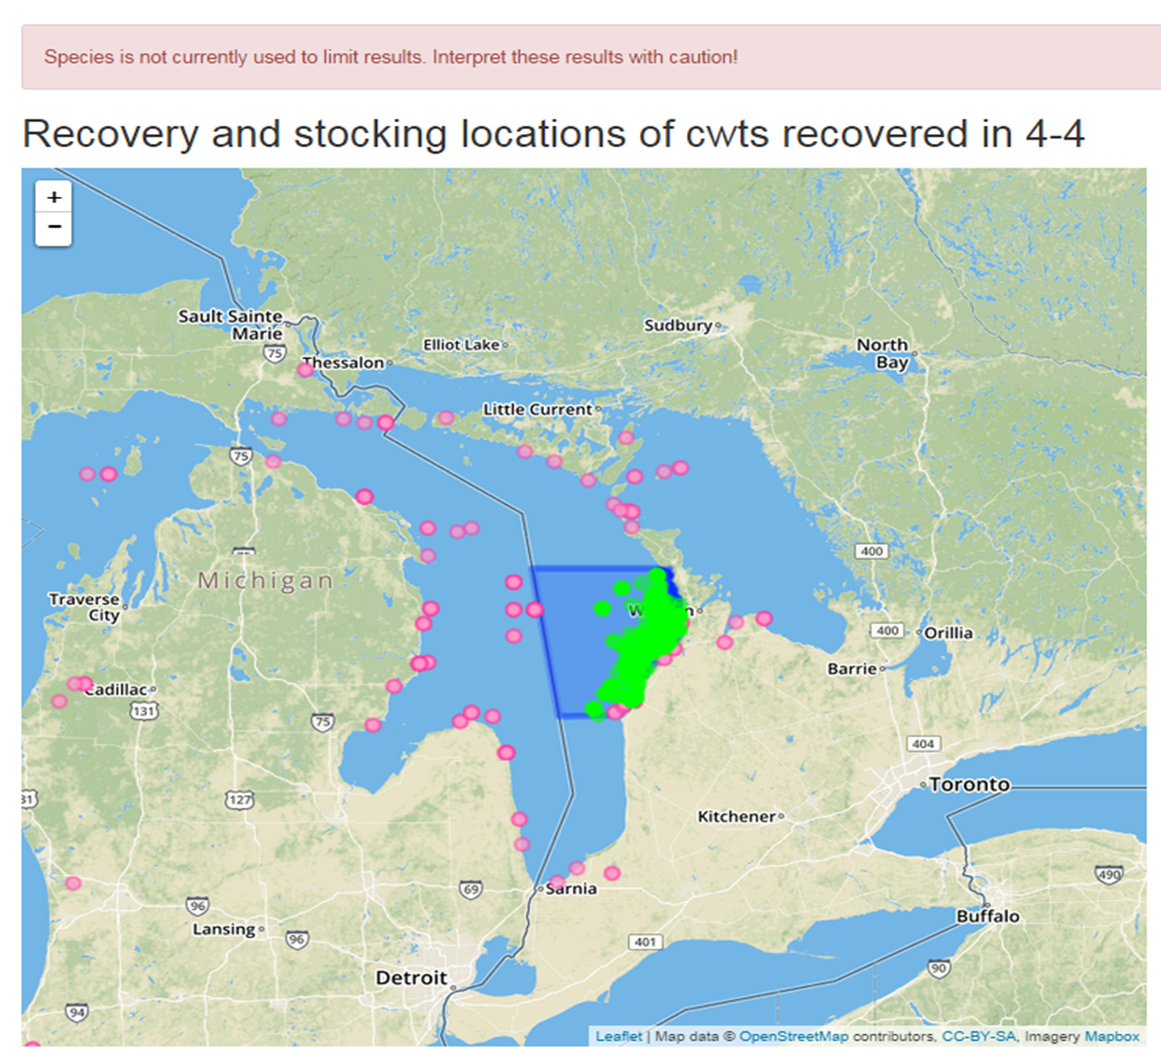
\includegraphics[width=0.9\textwidth]{caution}}
\end{column}
\end{columns}
\end{frame}
% Emacs 24.3.1 (Org mode 8.2.10)
\end{document}
